\documentclass[12pt,a4paper]{article}
\usepackage[utf8]{inputenc}
\usepackage[T1]{fontenc}
\usepackage{amsmath}
\usepackage{amssymb}
\usepackage{graphicx}
\usepackage[siunitx, americanvoltages]{circuitikz}
\author{Athul}
\begin{document}
	\ctikzset{bipoles/length=2cm}
	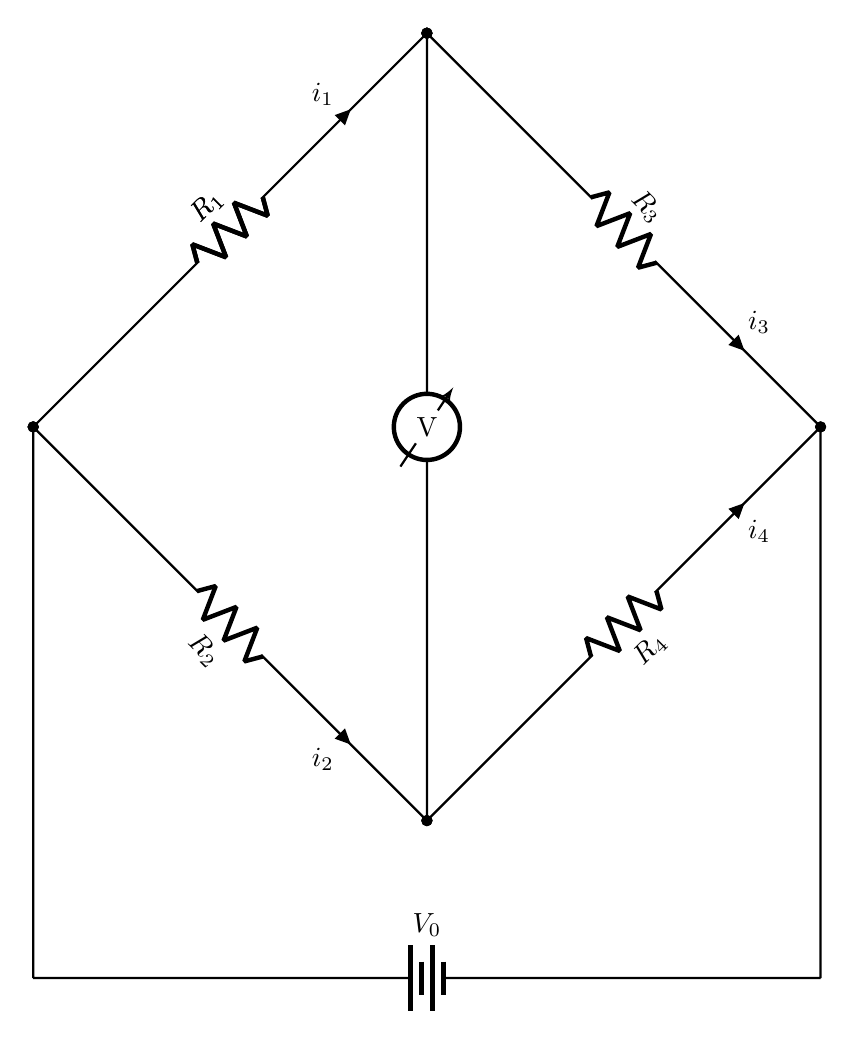
\begin{tikzpicture}[american]
		\draw[color=black, thick]
		(0,0) to [R,i>=$i_1$, l=$R_1$, *-*] (5,5)
		(5,5) to [R,i=$i_3$, l=$R_3$, *-*] (10,0) -- (10,-7)
		(10,0) to [R,i<=$i_4$, l=$R_4$, *-*] (5,-5)
		(5,-5) to [R,i<=$i_2$, l=$R_2$, *-*] (0,0) -- (0,-7)
		(5,-5) to [rmeterwa, t=V, *-*] (5,5)
		(0,0) to [R, l=$R_1$, *-*] (5,5)
		(0,-7) to [battery, l=$V_0$, -] (10,-7);
	\end{tikzpicture}
\end{document}